%%%%%%%%%%%%%%%%%%%%% chapter.tex %%%%%%%%%%%%%%%%%%%%%%%%%%%%%%%%%
%
% sample chapter
%
% Use this file as a template for your own input.
%
%%%%%%%%%%%%%%%%%%%%%%%% Springer-Verlag %%%%%%%%%%%%%%%%%%%%%%%%%%
%\motto{Use the template \emph{chapter.tex} to style the various elements of your chapter content.}

\chapter{Rosetta Code Tasks starting with D}

\section*{Date format}


This task has been clarified. Its programming examples are in need of
review to ensure that they still fit the requirements of the task.

Display the current date in the formats of ``2007-11-10'' and ``Sunday,
November 10, 2007''.

\begin{wideverbatim}

(let (Date (date)  Lst (date Date))
   (prinl (dat\$ Date "-"))             # 2010-02-19
   (prinl                              # Friday, February 19, 2010
      (day Date)
      ", "
      (get *MonFmt (cadr Lst))
      " "
      (caddr Lst)
      ", "
      (car Lst) ) )

\end{wideverbatim}

\pagebreak{}
\section*{Date manipulation}

Given the date string ``March 7 2009 7:30pm EST'', output the time 12
hours later in any human-readable format.

As extra credit, display the resulting time in a time zone different
from your own.

\begin{wideverbatim}

(de timePlus12 (Str)
   (use (@Mon @Day @Year @Time @Zone)
      (and
         (match
            '(@Mon " " @Day " " @Year " " @Time " " @Zone)
            (chop Str) )
         (setq @Mon (index (pack @Mon) *MonFmt))
         (setq @Day (format @Day))
         (setq @Year (format @Year))
         (setq @Time
            (case (tail 2 @Time)
               (("a" "m") (\$tim (head -2 @Time)))
               (("p" "m") (+ `(time 12 0) (\$tim (head -2 @Time))))
               (T (\$tim @Time)) ) )
         (let? Date (date @Year @Mon @Day)
            (when (>= (inc '@Time `(time 12 0)) 86400)
               (dec '@Time 86400)
               (inc 'Date) )
            (pack (dat\$ Date "-") " " (tim\$ @Time T) " " @Zone) ) ) ) )

\end{wideverbatim}

\pagebreak{}
\section*{Day of the week}

A company decides that whenever Xmas falls on a Sunday they will give
their workers all extra paid holidays so that, together with any public
holidays, workers will not have to work the following week (between the
25th of December and the first of January).

\textbf{In what years between 2008 and 2121 will the 25th of December be
a Sunday?}

Using any standard date handling libraries of your programming language;
compare the dates calculated with the output of other languages to
discover any anomalies in the handling of dates which may be due to, for
example, overflow in types used to represent dates/times similar to
\href{http://en.wikipedia.org/wiki/Y2k\#See\_also}{y2k} type problems.


\begin{wideverbatim}

(for (Y 2008 (>= 2121 Y) (inc Y))
   (when (= "Sunday" (day (date Y 12 25)))
      (printsp Y) ) )

Output:

2011 2016 2022 2033 2039 2044 2050 2061 2067 2072 2078 2089 2095 2101 2107 2112 2118

\end{wideverbatim}

\pagebreak{}
\section*{Deal cards for FreeCell}

\emph{Free Cell} is the solitaire card game that Paul Alfille
introduced to the PLATO system in 1978. Jim Horne, at Microsoft,
changed the name to \emph{FreeCell} and reimplemented the game for
\emph{DOS}, then \emph{Windows}. This version introduced 32000
numbered deals. (The
\href{http://www.solitairelaboratory.com/fcfaq.html}{FreeCell FAQ}
tells this history.)

As the game became popular, Jim Horne disclosed
\href{http://www.solitairelaboratory.com/mshuffle.txt}{the algorithm},
and other implementations of FreeCell began to reproduce the Microsoft
deals. These deals are numbered from 1 to 32000. Newer versions from
Microsoft have 1 million deals, numbered from 1 to 1000000; some
implementations allow numbers outside that range.

The algorithm uses this \emph{linear congruential generator} from
Microsoft C:

\begin{itemize}
\item
  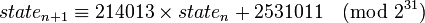
\includegraphics[scale=.6]{graphics/47c16228f3793455eb3436c78d21477d.png}
\item
  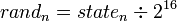
\includegraphics[scale=.6]{graphics/a026db06e1a9bd6945c85c8e17231725.png}
\item
  \emph{r}\emph{a}\emph{n}\emph{d}\textsubscript{\emph{n}} is in range 0
  to 32767.
\item Rosetta Code has another task, \emph{linear congruential
    generator}, with code for this RNG in several languages.
\end{itemize}

The algorithm follows:

\begin{enumerate}
\item
  Seed the RNG with the number of the deal.
\item
  Create an \emph{array} of 52 cards: Ace of Clubs, Ace of
  Diamonds, Ace of Hearts, Ace of Spades, 2 of Clubs, 2 of Diamonds, and
  so on through the ranks: Ace, 2, 3, 4, 5, 6, 7, 8, 9, 10, Jack, Queen,
  King. The array indexes are 0 to 51, with Ace of Clubs at 0, and King
  of Spades at 51.
\item
  Until the array is empty:

  \begin{itemize}
  \item
    Choose a random card at \emph{index} ≡ \emph{next random number}
    (mod \emph{array length}).
  \item
    Swap this random card with the last card of the array.
  \item
    Remove this random card from the array. (Array length goes down by
    1.)
  \item
    Deal this random card.
  \end{itemize}
\item
  Deal all 52 cards, face up, across 8 columns. The first 8 cards go in
  8 columns, the next 8 cards go on the first 8 cards, and so on.
\end{enumerate}

\pagebreak{}
\begin{verbatim}
Order to deal cards

 1  2  3  4  5  6  7  8
 9 10 11 12 13 14 15 16
17 18 19 20 21 22 23 24
25 26 27 28 29 30 31 32
33 34 35 36 37 38 39 40
41 42 43 44 45 46 47 48
49 50 51 52
\end{verbatim}

\begin{verbatim}
Game \#1

JD 2D 9H JC 5D 7H 7C 5H
KD KC 9S 5S AD QC KH 3H
2S KS 9D QD JS AS AH 3C
4C 5C TS QH 4H AC 4D 7S
3S TD 4S TH 8H 2C JH 7D
6D 8S 8D QS 6C 3D 8C TC
6S 9C 2H 6H
\end{verbatim}

\begin{verbatim}
Game \#617

7D AD 5C 3S 5S 8C 2D AH
TD 7S QD AC 6D 8H AS KH
TH QC 3H 9D 6S 8D 3D TC
KD 5H 9S 3C 8S 7H 4D JS
4C QS 9C 9H 7C 6H 2C 2S
4S TS 2H 5D JC 6C JH QH
JD KS KC 4H
\end{verbatim}

Deals can also be checked against
\href{http://freecellgamesolutions.com/}{FreeCell solutions to 1000000
  games}. (Summon a video solution, and it displays the initial deal.)

Write a program to take a deal number and deal cards in the same order
as this algorithm. The program may display the cards with ASCII, with
Unicode, by drawing graphics, or any other way.


\begin{wideverbatim}

Using the random generator from [[Linear congruential generator#PicoLisp]]:

(setq *MsSeed 11982)

(de msRand ()
   (>> 16
      (setq *MsSeed
         (\& (+ 2531011 (* 214013 *MsSeed)) `(dec (** 2 31))) ) ) )

(let L
   (make
      (for Num (range 13 1)
         (for Suit '((32 . "♠") (31 . "♥") (31 . "♦") (32 . "♣"))
            (link (cons (get '`(chop "A23456789TJQK") Num) Suit)) ) ) )
   (for I 51
      (xchg
         (nth L I)
         (nth L (- 52 (\% (msRand) (- 53 I)))) ) )
   (for C L
      (prin "  ^[[" (cadr C) "m" (cddr C) "^[[m" (car C))
      (at (0 . 8) (prinl)) )
   (prinl) )

\end{wideverbatim}

\pagebreak{}
\section*{Decision tables}

\href{http://en.wikipedia.org/wiki/Decision\_table}{Decision Tables} are
a precise yet compact way to model complicated logic. Demonstrate how
your language implements decision tables. Use the example of Printer
Troubleshooting given in the Wikipedia article.

\begin{wideverbatim}

We allow ourselves a luxurious user interface:

(de yes? (Cond)
   (out NIL (prin (car Cond) "? "))
   (in NIL
      (use Reply
         (loop
            (setq Reply (read))
            (T (member Reply '(T Y YES Yes y yes true 1))
               T )
            (T (member Reply '(NIL N NO No n no false 0)))
            (prinl "Please answer 'Yes' or 'No'") ) ) ) )

The decision table used in the example:

(de *Conditions
   ("Printer does not print"                T   T   T   T  NIL NIL NIL NIL)
   ("A red light is flashing"               T   T  NIL NIL  T   T  NIL NIL)
   ("Printer is unrecognised"               T  NIL  T  NIL  T  NIL  T  NIL) )

(de *Actions
   ("Check the power cable"                NIL NIL  T)
   ("Check the printer-computer cable"      T  NIL  T)
   ("Ensure printer software is installed"  T  NIL  T  NIL  T  NIL  T)
   ("Check/replace ink"                     T   T  NIL NIL  T   T)
   ("Check for paper jam"                  NIL  T  NIL  T) )

The decision can be made directly on the condition and action data, without the
need to create intermediate tables:

(de decide ()
   (let Reply (mapcar yes? *Conditions)
      (extract and
         (apply pick (append *Conditions *Actions)
            '(@
               (unless (pick '((Flg) (<> Flg (next))) Reply)
                  (rest) ) ) )
         (mapcar car *Actions) ) ) )


\end{wideverbatim}

\begin{wideverbatim}

Output:

: (decide)
Printer does not print? y
A red light is flashing? y
Printer is unrecognised? n
-> ("Check/replace ink" "Check for paper jam")

: (decide)
Printer does not print? n
A red light is flashing? y
Printer is unrecognised? y
-> ("Ensure printer software is installed" "Check/replace ink")

: (decide)
Printer does not print? n
A red light is flashing? n
Printer is unrecognised? n
-> NIL

\end{wideverbatim}


\pagebreak{}
\section*{Deconvolution/1D}

The convolution of two functions \emph{F} and \emph{H} of an integer
variable is defined as the function \emph{G} satisfying

\begin{figure}[H]
\centering
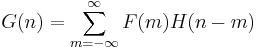
\includegraphics[scale=.6]{graphics/e4e4d6b17e1e15dbddc307340f0a620f.png}
% \caption{ G(n) =
% \textbackslash{}sum\_\{m=-\textbackslash{}infty\}\^{}\{\textbackslash{}infty\}
% F(m) H(n-m) }
\end{figure}

for all integers \emph{n}. Assume \emph{F}(\emph{n}) can be non-zero
only for 0 ≤ \emph{n} ≤ \textbar{} \emph{F} \textbar{} , where
\textbar{} \emph{F} \textbar{} is the ``length'' of \emph{F}, and
similarly for \emph{G} and \emph{H}, so that the functions can be
modeled as finite sequences by identifying

\includegraphics[scale=.6]{graphics/b14d36d888dae449d5c4fcfb6f4ff8ce.png}
with

\includegraphics[scale=.6]{graphics/2eb0e52a9d4ca2a57f0a0ceaca866399.png},
etc. Then for example, values of \textbar{} \emph{F} \textbar{} = 6 and
\textbar{} \emph{H} \textbar{} = 5 would determine the following value
of \emph{g} by definition.

\begin{figure}[H]
\centering
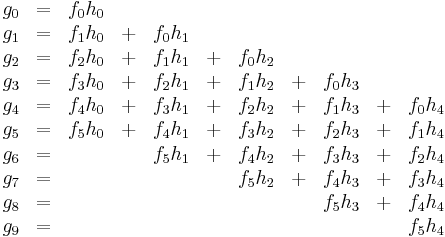
\includegraphics[scale=.6]{graphics/7f867e9ec901e62d2c8efa1ec9b4c5d6.png}
% \caption{ \textbackslash{}begin\{array\}\{lllllllllll\} g\_0 \&=
% \&f\_0h\_0\textbackslash{}\textbackslash{} g\_1 \&= \&f\_1h\_0 \&+
% \&f\_0h\_1\textbackslash{}\textbackslash{} g\_2 \&= \&f\_2h\_0 \&+
% \&f\_1h\_1 \&+ \&f\_0h\_2\textbackslash{}\textbackslash{} g\_3 \&=
% \&f\_3h\_0 \&+ \&f\_2h\_1 \&+ \&f\_1h\_2 \&+
% \&f\_0h\_3\textbackslash{}\textbackslash{} g\_4 \&= \&f\_4h\_0 \&+
% \&f\_3h\_1 \&+ \&f\_2h\_2 \&+ \&f\_1h\_3 \&+
% \&f\_0h\_4\textbackslash{}\textbackslash{} g\_5 \&= \&f\_5h\_0 \&+
% \&f\_4h\_1 \&+ \&f\_3h\_2 \&+ \&f\_2h\_3 \&+
% \&f\_1h\_4\textbackslash{}\textbackslash{} g\_6 \&= \& \& \&f\_5h\_1 \&+
% \&f\_4h\_2 \&+ \&f\_3h\_3 \&+ \&f\_2h\_4\textbackslash{}\textbackslash{}
% g\_7 \&= \& \& \& \& \&f\_5h\_2 \&+ \&f\_4h\_3 \&+
% \&f\_3h\_4\textbackslash{}\textbackslash{} g\_8 \&= \& \& \& \& \& \&
% \&f\_5h\_3 \&+ \&f\_4h\_4\textbackslash{}\textbackslash{} g\_9 \&= \& \&
% \& \& \& \& \& \& \&f\_5h\_4 \textbackslash{}end\{array\} }
\end{figure}

We can write this in matrix form as:

\begin{figure}[H]
\centering
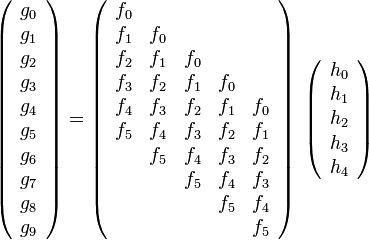
\includegraphics[scale=.6]{graphics/5cec990b9d6c1fdc3b340a364729aea6.png}
% \caption{ \textbackslash{}left( \textbackslash{}begin\{array\}\{l\} g\_0
% \textbackslash{}\textbackslash{} g\_1 \textbackslash{}\textbackslash{}
% g\_2 \textbackslash{}\textbackslash{} g\_3
% \textbackslash{}\textbackslash{} g\_4 \textbackslash{}\textbackslash{}
% g\_5 \textbackslash{}\textbackslash{} g\_6
% \textbackslash{}\textbackslash{} g\_7 \textbackslash{}\textbackslash{}
% g\_8 \textbackslash{}\textbackslash{} g\_9
% \textbackslash{}\textbackslash{} \textbackslash{}end\{array\}
% \textbackslash{}right) = \textbackslash{}left(
% \textbackslash{}begin\{array\}\{lllll\}
% f\_0\textbackslash{}\textbackslash{} f\_1 \&
% f\_0\textbackslash{}\textbackslash{} f\_2 \& f\_1 \&
% f\_0\textbackslash{}\textbackslash{} f\_3 \& f\_2 \& f\_1 \&
% f\_0\textbackslash{}\textbackslash{} f\_4 \& f\_3 \& f\_2 \& f\_1 \&
% f\_0\textbackslash{}\textbackslash{} f\_5 \& f\_4 \& f\_3 \& f\_2 \&
% f\_1\textbackslash{}\textbackslash{} \& f\_5 \& f\_4 \& f\_3 \&
% f\_2\textbackslash{}\textbackslash{} \& \& f\_5 \& f\_4 \&
% f\_3\textbackslash{}\textbackslash{} \& \& \& f\_5 \&
% f\_4\textbackslash{}\textbackslash{} \& \& \& \& f\_5
% \textbackslash{}end\{array\} \textbackslash{}right) \textbackslash{};
% \textbackslash{}left( \textbackslash{}begin\{array\}\{l\} h\_0
% \textbackslash{}\textbackslash{} h\_1 \textbackslash{}\textbackslash{}
% h\_2 \textbackslash{}\textbackslash{} h\_3
% \textbackslash{}\textbackslash{} h\_4 \textbackslash{}\textbackslash{}
% \textbackslash{}end\{array\} \textbackslash{}right) }
\end{figure}

or

\begin{figure}[H]
\centering
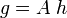
\includegraphics[scale=.6]{graphics/9321b2aa2a198225b0dbe56040b49940.png}
% \caption{ g = A \textbackslash{}; h }
\end{figure}

For this task, implement a function (or method, procedure, subroutine,
etc.) \texttt{deconv} to perform \emph{deconvolution} (i.e., the
\emph{inverse} of convolution) by constructing and solving such a system
of equations represented by the above matrix \emph{A} for \emph{h} given
\emph{f} and \emph{g}.

\begin{itemize}
\item
  The function should work for \emph{G} of arbitrary length (i.e., not
  hard coded or constant) and \emph{F} of any length up to that of
  \emph{G}. Note that \textbar{} \emph{H} \textbar{} will be given by
  \textbar{} \emph{G} \textbar{} − \textbar{} \emph{F} \textbar{} + 1.
\item There may be more equations than unknowns. If convenient, use a
  function from a
  \href{http://www.netlib.org/lapack/lug/node27.html}{library} that
  finds the best fitting solution to an overdetermined system of
  linear equations (as in the \emph{Multiple regression} task).
  Otherwise, prune the set of equations as needed and solve as in the
  \emph{Reduced row echelon form} task.
\item
  Test your solution on the following data. Be sure to verify both that
  \texttt{deconv}(\emph{g},\emph{f}) = \emph{h} and
  \texttt{deconv}(\emph{g},\emph{h}) = \emph{f} and display the results
  in a human readable form.
\end{itemize}

\begin{wideverbatim}

h = [-8,-9,-3,-1,-6,7] 

f = [-3,-6,-1,8,-6,3,-1,-9,-9,3,-2,5,2,-2,-7,-1]

g = [ 24,75,71,-34,3,22,-45,23,245,25,52,25,-67,-96,96,31,55,36,29,-43,-7]

\end{wideverbatim}

\begin{wideverbatim}

(load "@lib/math.l")
 
(de deconv (G F)
   (let A (pop 'F)
      (make
         (for (N . H) (head (- (length F)) G)
            (for (I . M) (made)
               (dec 'H
                  (*/ M (get F (- N I)) 1.0) ) )
            (link (*/ H 1.0 A)) ) ) ) )

Test:

(setq
   F (-3. -6. -1. 8. -6. 3. -1. -9. -9. 3. -2. 5. 2. -2. -7. -1.)
   G (24. 75. 71. -34. 3. 22. -45. 23. 245. 25. 52. 25. -67. -96.
   96. 31. 55. 36. 29. -43. -7.)
   H (-8. -9. -3. -1. -6. 7.) )
 
(test H (deconv G F))
(test F (deconv G H))

\end{wideverbatim}


\pagebreak{}
\section*{Deepcopy}

Demonstrate how to copy data structures containing complex
hetrogeneous and cyclic semantics. This is often referred to as
\href{http://en.wikipedia.org/wiki/Deep\_copy\#Deep\_copy}{deep
  copying}, and is normally required where structures are mutable and
to ensure that independent copies can be manipulated without
side-effects.

If this facility is not built into the language, it is permissible to
use functions from a common library, or a coded procedure.

The task should show:

\begin{itemize}
\item
  Relevant semantics of structures, such as their
  \href{http://en.wikipedia.org/wiki/Homogeneity\_and\_heterogeneity}{homogeneous
  or heterogeneous} properties, or containment of (self- or
  mutual-reference) cycles.
\end{itemize}

\begin{itemize}
\item
  Any limitations of the method.
\end{itemize}

\begin{itemize}
\item
  That the structure and its copy are different.
\end{itemize}

\begin{itemize}
\item
  Suitable links to external documentation for common libraries.

Show how to insert documentation for classes, functions, and/or
variables in your language. If this documentation is built-in to the
language, note it. If this documentation requires external tools, note
them.
\end{itemize}


\begin{wideverbatim}

A shallow copy can be done with '[http://software-lab.de/doc/refC.html#copy
copy]'. This function takes care of cons pairs and lists, no matter whether they
are cyclic, or end in NIL or some other data structure.

For a known depth, it might be used in combination with other list functions.
For example, to copy a non-cyclic structure of depth 2 with
'[http://software-lab.de/doc/refM.html#mapcar mapcar]':

(mapcar copy List)

Copying non-cyclic structures of arbitrary depth and list-termination could be
handled with a custom function (using
'[http://software-lab.de/doc/refC.html#cons cons]'):

(de deepCopy (X)
   (if (atom X)
      X
      (cons (deepCopy (car X)) (deepCopy (cdr X))) ) )

Test:

: (setq A '((a . b) (c d e) f g . e))
-> ((a . b) (c d e) f g . e)

: (setq B (deepCopy A))
-> ((a . b) (c d e) f g . e)

: A
-> ((a . b) (c d e) f g . e)

: B
-> ((a . b) (c d e) f g . e)

: (= A B)
-> T              # A and its copy B are structure-equal
: (== A B)
-> NIL            # but they are not identical (pointer-equal)

: (cadr A)
-> (c d e)

: (cadr B)
-> (c d e)

: (== (cadr A) (cadr B))
-> NIL            # The same holds for sub-structures

\end{wideverbatim}

\begin{wideverbatim}

For cyclic structures, the above 'deepCopy' function could be extended, to
remember already visited structures and their copies in a mark list:

(de deepCopy (X)
   (let Mark NIL
      (recur (X)
         (cond
            ((atom X) X)
            ((asoq X Mark) (cdr @))
            (T
               (prog1 (cons)
                  (push 'Mark (cons X @))
                  (set @ (recurse (car X)))
                  (con @ (recurse (cdr X))) ) ) ) ) ) )

Test:

: (setq A '(a b .)  B (deepCopy A))
-> (a b .)
: A
-> (a b .)
: B
-> (a b .)

: (= A B)
-> T              # A and its copy B are structure-equal

: (== A B)
-> NIL            # but they are not identical (pointer-equal)

\end{wideverbatim}

\pagebreak{}
\section*{Define a primitive data type}


Demonstrate how to define a type that behaves like an integer but has a
lowest valid value of 1 and a highest valid value of 10. Include all
bounds checking you need to write, or explain how the compiler or
interpreter creates those bounds checks for you.



\begin{wideverbatim}

(class +BoundedInt)
# value lower upper

(dm T (Low Up)
   (=: lower (min Low Up))
   (=: upper (max Low Up)) )

(de "checkBounds" (Val)
   (if (>= (: upper) Val (: lower))
      Val
      (throw 'boundedIntOutOfBounds
         (pack
            "value " Val
            " is out of bounds [" (: lower) "," (: upper) "]" ) ) ) )

(dm set> (Val)
   (=: value ("checkBounds" Val)) )

(dm +> (Val)
   (=: value ("checkBounds" (+ Val (: value)))) )

(dm val> ()
   (: value) )

(de main ()
   (let (A (new '(+BoundedInt) 1 10)  B (new '(+BoundedInt) 1 10))
      (set> A 6)
      (when (catch 'boundedIntOutOfBounds (set> B 12) NIL)
         (prinl @) )
      (set> B 9)
      (when (catch 'boundedIntOutOfBounds (+> A (val> B)) NIL)
         (prinl @) ) ) )

Output:

: (main)
value 12 is out of bounds [1,10]
value 15 is out of bounds [1,10]

\end{wideverbatim}

\pagebreak{}
\section*{Delegates}

A delegate is a helper object used by another object. The delegator may
send the delegate certain messages, and provide a default implementation
when there is no delegate or the delegate does not respond to a message.
This pattern is heavily used in
\href{http://developer.apple.com/documentation/Cocoa/Conceptual/CocoaFundamentals/CocoaDesignPatterns/chapter\_5\_section\_3.html\#//apple\_ref/doc/uid/TP40002974-CH6-DontLinkElementID\_93}{Cocoa
framework on Mac OS X}. See also
\href{http://en.wikipedia.org/wiki/Delegation\_pattern}{wp:Delegation
pattern}.

Objects responsibilities:

Delegator:

\begin{itemize}
\item
  Keep an optional delegate instance.
\item
  Implement ``operation'' method, returning the delegate ``thing'' if
  the delegate respond to ``thing'', or the string ``default
  implementation''.
\end{itemize}

Delegate:

\begin{itemize}
\item
  Implement ``thing'' and return the string ``delegate implementation''
\end{itemize}

Show how objects are created and used. First, without a delegate, then
with a delegate that does not implement ``thing'', and last with a
delegate that implements ``thing''.



\begin{wideverbatim}

(class +Delegator)
# delegate

(dm operation> ()
   (if (: delegate)
      (thing> @)
      "default implementation" ) )


(class +Delegate)
# thing

(dm T (Msg)
   (=: thing Msg) )

(dm thing> ()
   (: thing) )


(let A (new '(+Delegator))
   # Without a delegate
   (println (operation> A))

   # With delegate that does not implement 'thing>'
   (put A 'delegate (new '(+Delegate)))
   (println (operation> A))

   # With delegate that implements 'thing>'
   (put A 'delegate (new '(+Delegate) "delegate implementation"))
   (println (operation> A)) )

Output:

"default implementation"
NIL
"delegate implementation"

\end{wideverbatim}

\pagebreak{}
\section*{Delete a file}

In this task, the job is to delete a file called ``input.txt'' and
delete a directory called ``docs''. This should be done twice: once
``here'', i.e. in the current working directory and once in the
filesystem root.

\begin{wideverbatim}

(call 'rm "input.txt")
(call 'rmdir "docs")
(call 'rm "/input.txt")
(call 'rmdir "/docs")

\end{wideverbatim}

\pagebreak{}
\section*{Detect division by zero}

Write a function to detect a divide by zero error without checking if
the denominator is zero.

\begin{wideverbatim}

(catch '("Div/0") (/ A B))

\end{wideverbatim}

\pagebreak{}
\section*{Determine if a string is numeric}

Create a boolean function which takes in a string and tells whether it
is a numeric string (floating point and negative numbers included) in
the syntax the language uses for numeric literals or numbers converted
from strings.

\begin{wideverbatim}

  The 'format' function can be used for that. It returns NIL if the
  given string is not a legal number

: (format "123")
-> 123

: (format "123a45")
-> NIL

: (format "-123.45" 4)
-> 1234500

\end{wideverbatim}

\pagebreak{}
\section*{Determine if only one instance is running}

This task is to determine if there is only one instance of an
application running. If the program discovers that an instance of it is
already running, then it should display a message indicating that it is
already running and exit.


\begin{wideverbatim}

Calling 'killall'

One possibility is to send a zero-signal with 'killall', and check the return
value. This is useful if each application is started by a hash-bang script (the
first line is e.g. "#!/usr/bin/picolisp /usr/lib/picolisp/lib.l"). In that way,
each application has its own name which can be passed to 'killall'.

\$ cat myScript
#!/usr/bin/picolisp /usr/lib/picolisp/lib.l

(wait 120000)
(bye)

\$ ./myScript \&  # Start in the background
[1] 26438

\$ pil +
: (call "killall" "-0" "-q" "myScript")
-> T

Using a mutex

Another possibility is to 'acquire' a mutex on program start, and never release
it.

: (acquire "running1")
-> 30817  # A successful call returns the PID

A second application trying to acquire the same mutex would receive 'NIL'

\end{wideverbatim}

% \pagebreak{}
% \section*{Determine the maximum height and width of a window}

% \begin{wideverbatim}

% The following works on ErsatzLisp, the Java version of PicoLisp.

% (let Frame (java "javax.swing.JFrame" T "Window")
%    (java Frame 'setExtendedState
%       (java (public "javax.swing.JFrame" 'MAXIMIZED_BOTH)) )
%    (java Frame 'setVisible T)
%    (wait 200)
%    (let Size (java (java Frame 'getContentPane) 'getSize)
%       (prinl "Width: " (java (public Size 'width)))
%       (prinl "Height: " (java (public Size 'height))) )
%    (java Frame 'dispose) )

% Output (on a 1024x768 screen):

% Width: 1010
% Height: 735

% \end{wideverbatim}


\pagebreak{}
\section*{Digital root}

Related task \emph{Sum digits of an integer}

The digital root (X) of a number (N) is calculated:

find X as the sum of the digits of N

find a new X by summing the digits of X repeating until X has only one
digit.

The additive persistance is the number of summations required to obtain
the single digit.

The task is to calculate the additive persistance and the digital root
of a number. e.g.

627615 has additive persistance 2 and digital root of 9;

39390 has additive persistance 2 and digital root of 6;

588225 has additive persistance 2 and digital root of 3;

393900588225 has additive persistance 2 and digital root of 9;

The digital root may be calculated in bases other than 10.

See: \emph{Casting out nines} for this wiki's use of this procedure.


\begin{wideverbatim}

(for N (627615 39390 588225 393900588225)
   (for ((A . I) N  T  (sum format (chop I)))
      (T (> 10 I)
         (prinl N " has additive persistance " (dec A) " and digital root of " I ";") ) ) )

Output:

627615 has additive persistance 2 and digital root of 9;
39390 has additive persistance 2 and digital root of 6;
588225 has additive persistance 2 and digital root of 3;
393900588225 has additive persistance 2 and digital root of 9;

\end{wideverbatim}

\pagebreak{}
\section*{Dijkstra's algorithm}

\textbf{Dijkstra's algorithm}, conceived by Dutch computer scientist
\href{http://en.wikipedia.org/wiki/Edsger\_Dijkstra}{Edsger Dijkstra} in
1956 and published in 1959, is a
\href{http://en.wikipedia.org/wiki/graph\_search\_algorithm}{graph
search algorithm} that solves the single-source
\href{http://en.wikipedia.org/wiki/shortest\_path\_problem}{shortest
path problem} for a
\href{http://en.wikipedia.org/wiki/graph\_(mathematics)}{graph} with
nonnegative
\href{http://en.wikipedia.org/wiki/edge\_(graph\_theory)}{edge} path
costs, producing a
\href{http://en.wikipedia.org/wiki/shortest\_path\_tree}{shortest path
tree}. This algorithm is often used in
\href{http://en.wikipedia.org/wiki/routing}{routing} and as a subroutine
in other graph algorithms.

For a given source
\href{http://en.wikipedia.org/wiki/vertex\_(graph\_theory)}{vertex}
(node) in the graph, the algorithm finds the path with lowest cost (i.e.
the shortest path) between that vertex and every other vertex. It can
also be used for finding costs of shortest paths from a single vertex to
a single destination vertex by stopping the algorithm once the shortest
path to the destination vertex has been determined. For example, if the
vertices of the graph represent cities and edge path costs represent
driving distances between pairs of cities connected by a direct road,
Dijkstra's algorithm can be used to find the shortest route between one
city and all other cities. As a result, the shortest path first is
widely used in network
\href{http://en.wikipedia.org/wiki/routing\_protocol}{routing
protocols}, most notably
\href{http://en.wikipedia.org/wiki/IS-IS}{IS-IS} and
\href{http://en.wikipedia.org/wiki/OSPF}{OSPF} (Open Shortest Path
First).

\textbf{Task:}

\begin{enumerate}
\item
  Implement a version of Dijkstra's algorithm that computes a shortest
  path from a start vertex to an end vertex in a directed graph.
\item
  Run your program with the following directed graph to find the
  shortest path from vertex ``a'' to vertex ``e.''
\item
  Show the output of your program.
\end{enumerate}

\ctable[caption = { Vertices }, pos = H, center, botcap]{ll}
{% notes
}
{% rows
\FL
Number & Name
\ML
1 & a
\\\noalign{\medskip}
2 & b
\\\noalign{\medskip}
3 & c
\\\noalign{\medskip}
4 & d
\\\noalign{\medskip}
5 & e
\\\noalign{\medskip}
6 & f
\LL
}

\ctable[caption = { Edges }, pos = H, center, botcap]{lll}
{% notes
}
{% rows
\FL
Start & End & Cost
\ML
a & b & 7
\\\noalign{\medskip}
a & c & 9
\\\noalign{\medskip}
a & f & 14
\\\noalign{\medskip}
b & c & 10
\\\noalign{\medskip}
b & d & 15
\\\noalign{\medskip}
c & d & 11
\\\noalign{\medskip}
c & f & 2
\\\noalign{\medskip}
d & e & 6
\\\noalign{\medskip}
e & f & 9
\LL
}

You can use numbers or names to identify vertices in your program.

\textbf{Extra Credit:} Document the specific algorithm implemented. The
\{\{trans\}\} template is sufficient. Otherwise add text outside of your
program or add comments within your program. This is not a requirement
to explain \emph{how} the algorithm works, but to state \emph{which}
algorithm is implemented. If your code follows an external source such
as the Wikipedia pseudocode, you can state that. You can state if it is
Dijkstra's original algorithm or some more efficient variant. It is
relevant to mention things like priority queues, heaps, and expected
time complexity in big-O notation. If a priority queue is used, it is
important to discuss how the step of decreasing the distance of a node
is accomplished, and whether it is linear or logarithmic time.



\begin{wideverbatim}
Following the Wikipedia algorithm:

(de neighbor (X Y Cost)
   (push (prop X 'neighbors) (cons Y Cost))
   (push (prop Y 'neighbors) (cons X Cost)) )
 
(de dijkstra (Curr Dest)
   (let Cost 0
      (until (== Curr Dest)
         (let (Min T  Next)
            (for N (; Curr neighbors)
               (with (car N)
                  (let D (+ Cost (cdr N))
                     (unless (and (: distance) (>= D @))
                        (=: distance D) ) )
                  (when (> Min (: distance))
                     (setq Min (: distance)  Next This) )
                  (del (asoq Curr (: neighbors)) (:: neighbors)) ) )
            (setq Curr Next  Cost Min) ) )
      Cost ) )

Test:

(neighbor 'a 'b 7)
(neighbor 'a 'c 9)
(neighbor 'a 'f 14)
(neighbor 'b 'c 10)
(neighbor 'b 'd 15)
(neighbor 'c 'd 11)
(neighbor 'c 'f 2)
(neighbor 'd 'e 6)
(neighbor 'e 'f 9)
 
(dijkstra 'a 'e)

Output:

-> 20

\end{wideverbatim}

\pagebreak{}
\section*{Dinesman's multiple-dwelling problem}

The task is to \textbf{solve Dinesman's multiple dwelling
\href{http://www-mitpress.mit.edu/sicp/full-text/book/book-Z-H-28.html\#\%\_sec\_4.3.2}{problem}
but in a way that most naturally follows the problem statement given
below}. Solutions are allowed (but not required) to parse and interpret
the problem text, but should remain flexible and should state what
changes to the problem text are allowed. Flexibility and ease of
expression are valued.

Examples may be be split into ``setup'', ``problem statement'', and
``output'' sections where the ease and naturalness of stating the
problem and getting an answer, as well as the ease and flexibility of
modifying the problem are the primary concerns.

Example output should be shown here, as well as any comments on the
examples flexibility.

\textbf[The problem] 

\emph{Baker, Cooper, Fletcher, Miller, and Smith live on different
floors of an apartment house that contains only five floors. Baker does
not live on the top floor. Cooper does not live on the bottom floor.
Fletcher does not live on either the top or the bottom floor. Miller
lives on a higher floor than does Cooper. Smith does not live on a floor
adjacent to Fletcher's. Fletcher does not live on a floor adjacent to
Cooper's. Where does everyone live?}


\begin{wideverbatim}

Using Pilog (PicoLisp Prolog). The problem can be modified by changing just the
'dwelling' rule (the "Problem statement"). This might involve the names and
number of dwellers (the list in the first line), and statements about who does
(or does not) live on the top floor (using the 'topFloor' predicate), the bottom
floor (using the 'bottomFloor' predicate), on a higher floor (using the
'higherFloor' predicate) or on an adjecent floor (using the 'adjacentFloor'
predicate). The logic follows an implied AND, and statements may be arbitrarily
combined using OR and NOT (using the 'or' and 'not' predicates), or any other
Pilog (Prolog) built-in predicates. If the problem statement has several
solutions, they will be all generated.

# Problem statement
(be dwelling (@Tenants)
   (permute (Baker Cooper Fletcher Miller Smith) @Tenants)
   (not (topFloor Baker @Tenants))
   (not (bottomFloor Cooper @Tenants))
   (not (or ((topFloor Fletcher @Tenants)) ((bottomFloor Fletcher @Tenants))))
   (higherFloor Miller Cooper @Tenants)
   (not (adjacentFloor Smith Fletcher @Tenants))
   (not (adjacentFloor Fletcher Cooper @Tenants)) )

# Utility rules
(be topFloor (@Tenant @Lst)
   (equal (@ @ @ @ @Tenant) @Lst) )

(be bottomFloor (@Tenant @Lst)
   (equal (@Tenant @ @ @ @) @Lst) )

(be higherFloor (@Tenant1 @Tenant2 @Lst)
   (append @ @Rest @Lst)
   (equal (@Tenant2 . @Higher) @Rest)
   (member @Tenant1 @Higher) )

(be adjacentFloor (@Tenant1 @Tenant2 @Lst)
   (append @ @Rest @Lst)
   (or
      ((equal (@Tenant1 @Tenant2 . @) @Rest))
      ((equal (@Tenant2 @Tenant1 . @) @Rest)) ) )

Output:

: (? (dwelling @Result))
 @Result=(Smith Cooper Baker Fletcher Miller)  # Only one solution
-> NIL

\end{wideverbatim}

\pagebreak{}
\section*{Dining philosophers}

The dining philosophers problem illustrates non-composability of
low-level synchronization primitives like
\emph{semaphores}. It is a modification of a problem
posed by Edsger Dijkstra.

Five philosophers, Aristotle, Kant, Spinoza, Marx, and Russell (the
\emph{tasks}) spend their time thinking and eating spaghetti. They eat
at a round table with five individual seats. For eating each
philosopher needs two forks (the resources). There are five forks on
the table, one left and one right of each seat. When a philosopher
cannot grab both forks it sits and waits. Eating takes random time,
then the philosopher puts the forks down and leaves the dining room.
After spending some random time thinking about the nature of the
universe, he again becomes hungry, and the circle repeats itself.

It can be observed that a straightforward solution, when forks are
implemented by \emph{semaphores}, is exposed to deadlock. There exist
two deadlock states when all five philosophers are sitting at the
table holding one fork each. One deadlock state is when each
philosopher has grabbed the fork left of him, and another is when each
has the fork on his right.

There are many solutions of the problem, program at least one, and
explain how the deadlock is prevented.


\begin{wideverbatim}

This following solution uses the built-in fininte state machine function
'[http://software-lab.de/doc/refS.html#state state]'. Deadlocks are avoided, as
each philosopher releases the first fork if he doesn't succeed to obtain the
second fork, and waits for a random time.

Another solution, using the Chandy/Misra method, can be found
[http://logand.com/sw/phil.l here].

(de dining (Name State)
   (loop
      (prinl Name ": " State)
      (state 'State                       # Dispatch according to state
         (thinking 'hungry)               # If thinking, get hungry
         (hungry                          # If hungry, grab random fork
            (if (rand T)
               (and (acquire leftFork) 'leftFork)
               (and (acquire rightFork) 'rightFork) ) )
         (hungry 'hungry                  # Failed, stay hungry for a while
            (wait (rand 1000 3000)) )
         (leftFork                        # If holding left fork, try right one
            (and (acquire rightFork) 'eating)
            (wait 2000) )                 # then eat for 2 seconds
         (rightFork                       # If holding right fork, try left one
            (and (acquire leftFork) 'eating)
            (wait 2000) )                 # then eat for 2 seconds
         ((leftFork rightFork) 'hungry    # Otherwise, go back to hungry,
            (release (val State))         # release left or right fork
            (wait (rand 1000 3000)) )     # and stay hungry
         (eating 'thinking             # After eating, resume thinking
            (release leftFork)
            (release rightFork)
            (wait 6000) ) ) ) )           # for 6 seconds
 
(setq *Philosophers
   (maplist
      '((Phils Forks)
         (let (leftFork (tmp (car Forks))  rightFork (tmp (cadr Forks)))
            (or
               (fork)  # Parent: Collect child process IDs
               (dining (car Phils) 'hungry) ) ) )  # Initially hungry
      '("Aristotle" "Kant" "Spinoza" "Marx" "Russell")
      '("ForkA" "ForkB" "ForkC" "ForkD" "ForkE" .) ) )
 
(push '*Bye '(mapc kill *Philosophers))  # Terminate all upon exit

\end{wideverbatim}

\begin{wideverbatim}

Output:

<pre>Aristotle: hungry
Aristotle: rightFork
Kant: hungry
Kant: rightFork
Spinoza: hungry
Spinoza: rightFork
Marx: hungry
Marx: rightFork
Russell: hungry
Marx: hungry
Spinoza: hungry
Kant: hungry
Russell: hungry
Aristotle: eating
...

\end{wideverbatim}

\pagebreak{}
\section*{Discordian date}

Convert a given date from the Gregorian calendar to the Discordian
calendar.

\textbf{See Also}

\begin{itemize}
\item
  \href{http://en.wikipedia.org/wiki/Discordian\_calendar}{Discordian
  calendar (wiki)}
\end{itemize}


\begin{wideverbatim}

(de disdate (Year Month Day)
   (let? Date (date Year Month Day)
      (let (Leap (date Year 2 29)  D (- Date (date Year 1 1)))
         (if (and Leap (= 2 Month) (= 29 Day))
            (pack "St. Tib's Day, YOLD " (+ Year 1166))
            (and Leap (>= D 60) (dec 'D))
            (pack
               (get
                  '("Chaos" "Discord" "Confusion" "Bureaucracy" "The Aftermath")
                  (inc (/ D 73)) )
               " "
               (inc (\% D 73))
               ", YOLD "
               (+ Year 1166) ) ) ) ) )

\end{wideverbatim}

\pagebreak{}
\section*{Distributed programming}

Write two programs (or one program with two modes) which run on
networked computers, and send some messages between them.

The protocol used may be language-specific or not, and should be
\textbf{suitable for general distributed programming}; that is, the
\emph{protocol} should be generic (not designed just for the particular
example application), readily capable of handling the independent
communications of many different components of a single application, and
the transferring of arbitrary data structures natural for the language.

This task is intended to demonstrate high-level communication
facilities beyond just creating \emph{sockets}.


\begin{wideverbatim}

# Server

(task (port 12321)                     # Background server task
   (let? Sock (accept @)
      (unless (fork)                   # Handle request in child process
         (in Sock
            (while (rd)                # Handle requests
               (out Sock
                  (pr (eval @)) ) ) )  # Evaluate and send reply
         (bye) )                       # Exit child process
      (close Sock) ) )                 # Close socket in parent process

# Client

(let? Sock (connect "localhost" 12321)
   (out Sock (pr '*Pid))               # Query PID from server
   (println 'PID (in Sock (rd)))       # Receive and print reply
   (out Sock (pr '(* 3 4)))            # Request some calculation
   (println 'Result (in Sock (rd)))    # Print result
   (close Sock) )                      # Close connection to server

Output:

PID 18372
Result 12

\end{wideverbatim}

\pagebreak{}
\section*{DNS query}

DNS is an internet service that maps domain names, like
\texttt{rosettacode.org}, to IP addresses, like \texttt{66.220.0.231}.

Use DNS to resolve \texttt{www.kame.net} to both IPv4 and IPv6
addresses. Print these addresses.


\begin{wideverbatim}

(make
   (in '(host "www.kame.net")
      (while (from "address ")
         (link (till "^J" T)) ) ) )

Output:

-> ("203.178.141.194" "2001:200:dff:fff1:216:3eff:feb1:44d7")

\end{wideverbatim}


\pagebreak{}
\section*{Documentation}

Show how to insert documentation for classes, functions, and/or
variables in your language. If this documentation is built-in to the
language, note it. If this documentation requires external tools, note
them.

\begin{wideverbatim}

PicoLisp doesn't yet support inline documentation directly in the code. However,
it has built-in runtime documentation via the
'[http://software-lab.de/doc/refD.html#doc doc]' function. This requires no
external tools, except that the interpreter must have been started in debug
mode.

: (doc 'car)         # View documentation of a function

: (doc '+Entity)     # View documentation of a class

: (doc '+ 'firefox)  # Explicitly specify a browser

\end{wideverbatim}

\pagebreak{}
\section*{Dot product}

Create a function/use an in-built function, to compute the
\textbf{\href{http://en.wikipedia.org/wiki/Dot\_product}{dot product}},
also known as the \textbf{scalar product} of two vectors. If possible,
make the vectors of arbitrary length.

As an example, compute the dot product of the vectors
\texttt{{[}1, 3, -5{]}} and \texttt{{[}4, -2, -1{]}}.

If implementing the dot product of two vectors directly, each vector
must be the same length; multiply corresponding terms from each vector
then sum the results to produce the answer.

\begin{description}
\item[Reference]
\end{description}

\begin{itemize}
\item \emph{Vector products} on Rosetta Code.
\end{itemize}


\begin{wideverbatim}

(de dotProduct (A B)
   (sum * A B) )

(dotProduct (1 3 -5) (4 -2 -1))

Output:

-> 3

\end{wideverbatim}

\pagebreak{}
\section*{Doubly-linked list/Definition}

Define the data structure for a complete Doubly Linked List.

\begin{itemize}
\item
  The structure should support adding elements to the head, tail and
  middle of the list.
\item
  The structure should not allow circular loops
\end{itemize}

See also \emph{Linked List}


\begin{wideverbatim}

For the list of double-cell structures described in
[[Doubly-linked list/Element definition#PicoLisp]],
we define a header structure, containing one pointer to the start
and one to the end of the list.

            +------------> start
            |
         +--+--+-----+
         |  |  |  ---+---> end
         +-----+-----+

# Build a doubly-linked list
(de 2list @
   (let Prev NIL
      (let L
         (make
            (while (args)
               (setq Prev (chain (list (next) Prev))) ) )
         (cons L Prev) ) ) )

(setq *DLst (2list 'was 'it 'a 'cat 'I 'saw))

For output of the example data, see [[Doubly-linked list/Traversal#PicoLisp]].

\end{wideverbatim}

\pagebreak{}
\section*{Doubly-linked list/Element definition}

Define the data structure for a \emph{doubly-linked list} element. The
element should include a data member to hold its value and pointers to
both the next element in the list and the previous element in the
list. The pointers should be mutable.

\begin{wideverbatim}

We use (in addition to the header structure described in
[[Doubly-linked list/Definition#PicoLisp]])
two cells per doubly-linked list element:

         +-----+-----+     +-----+-----+
         | Val |  ---+---> |  |  |  ---+---> next
         +-----+-----+     +--+--+-----+
                              |
                     prev <---+

With that, 'cddr' can be used to access the next, and 'cadr' to access the
previous element.

# 'cons' an element to a doubly-linked list
(de 2cons (X DLst)
   (let L (car DLst)                  # Get current data list
      (set DLst (cons X NIL L))       # Prepend two new cons pairs
      (if L                           # Unless DLst was empty
         (set (cdr L) (car DLst))     # set new 'prev' link
         (con DLst (car DLst)) ) ) )  # otherwise set 'end' link

# We prepend 'not' to the list in the previous example
(2cons 'not *DLst)

For output of the example data, see [[Doubly-linked list/Traversal#PicoLisp]].

\end{wideverbatim}

\pagebreak{}
\section*{Doubly-linked list/Element insertion}

Use the link structure defined in \emph{Doubly-Linked List (element)}
to define a procedure for inserting a link into a doubly-linked list.
Call this procedure to insert element C into a list \{A,B\}, between
elements A and B.

This is much like inserting into a \emph{Singly-Linked List}, but with
added assignments so that the backwards-pointing links remain correct.


\begin{wideverbatim}

This works with the structures described in
[[Doubly-linked list/Definition#PicoLisp]] and
[[Doubly-linked list/Element definition#PicoLisp]].

# Insert an element X at position Pos
(de 2insert (X Pos DLst)
   (let (Lst (nth (car DLst) (dec (* 2 Pos)))  New (cons X (cadr Lst) Lst))
      (if (cadr Lst)
         (con (cdr @) New)
         (set DLst New) )
      (if (cdr Lst)
         (set @ New)
         (con DLst New) ) ) )

(setq *DL (2list 'A 'B))      # Build a two-element doubly-linked list
(2insert 'C 2 *DL)            # Insert C at position 2

For output of the example data, see [[Doubly-linked list/Traversal#PicoLisp]].

\end{wideverbatim}

\pagebreak{}
\section*{Doubly-linked list/Traversal}

Traverse from the beginning of a
\href{/wiki/Doubly-linked\_list/Definition}{doubly-linked list} to the
end, and from the end to the beginning.


\begin{wideverbatim}

# Print the elements a doubly-linked list
(de 2print (DLst)
   (for (L (car DLst) L (cddr L))
      (printsp (car L)) )
   (prinl) )

# Print the elements a doubly-linked list in reverse order
(de 2printReversed (DLst)
   (for (L (cdr DLst) L (cadr L))
      (printsp (car L)) )
   (prinl) )

Output for the example data produced in
[[Doubly-linked list/Definition#PicoLisp]] and
[[Doubly-linked list/Element definition#PicoLisp]]:

: (2print *DLst)                 # Print the list
not was it a cat I saw

: (2printReversed *DLst)         # Print it in reversed order
saw I cat a it was not

Output for the example data produced in
[[Doubly-linked list/Element insertion#PicoLisp]]:

: (2print *DL)                   # Print the list
A C B

: (2printReversed *DL)           # Print it in reversed order
B C A

\end{wideverbatim}

\pagebreak{}
\section*{Dragon curve}

Create and display a
\href{http://en.wikipedia.org/wiki/dragon\_curve}{dragon curve}
fractal. (You may either display the curve directly or write it to an
image file.)


\begin{wideverbatim}

This uses the 'brez' line drawing function from
[[Bitmap/Bresenham's line algorithm#PicoLisp]].

# Need some turtle graphics
(load "@lib/math.l")

(setq
   *TurtleX 100      # X position
   *TurtleY  75      # Y position
   *TurtleA 0.0 )    # Angle

(de fd (Img Len)  # Forward
   (let (R (*/ *TurtleA pi 180.0)  DX (*/ (cos R) Len 1.0)  DY (*/ (sin R) Len 1.0))
      (brez Img *TurtleX *TurtleY DX DY)
      (inc '*TurtleX DX)
      (inc '*TurtleY DY) ) )

(de rt (A)  # Right turn
   (inc '*TurtleA A) )

(de lt (A)  # Left turn
   (dec '*TurtleA A) )


# Dragon curve stuff
(de *DragonStep . 4)

(de dragon (Img Depth Dir)
   (if (=0 Depth)
      (fd Img *DragonStep)
      (rt Dir)
      (dragon Img (dec Depth) 45.0)
      (lt (* 2 Dir))
      (dragon Img (dec Depth) -45.0)
      (rt Dir) ) )

# Run it
(let Img (make (do 200 (link (need 300 0))))       # Create image 300 x 200
   (dragon Img 10 45.0)                            # Build dragon curve
   (out "img.pbm"                                  # Write to bitmap file
      (prinl "P1")
      (prinl 300 " " 200)
      (mapc prinl Img) ) )

\end{wideverbatim}


\pagebreak{}
\section*{Draw a clock}

\textbf{Task}: draw a clock. More specific:

\begin{enumerate}
\item
  Draw a time keeping device. It can be a stopwatch, hourglass, sundial,
  a mouth counting ``one thousand and one'', anything. Only showing the
  seconds is required, e.g. a watch with just a second hand will
  suffice. However, it must clearly change every second, and the change
  must cycle every so often (one minute, 30 seconds, etc.) It must be
  \emph{drawn}; printing a string of numbers to your terminal doesn't
  qualify. Both text-based and graphical drawing are OK.
\item
  The clock is unlikely to be used to control space flights, so it needs
  not be hyper-accurate, but it should be usable, meaning if one can
  read the seconds off the clock, it must agree with the system clock.
\item
  A clock is rarely (never?) a major application: don't be a CPU hog and
  poll the system timer every microsecond, use a proper
  timer/signal/event from your system or language instead. For a bad
  example, many OpenGL programs update the framebuffer in a busy loop
  even if no redraw is needed, which is very undesirable for this task.
\item
  A clock is rarely (never?) a major application: try to keep your code
  simple and to the point. Don't write something too elaborate or
  convoluted, instead do whatever is natural, concise and clear in your
  language.
\end{enumerate}

Key points: animate simple object; timed event; polling system
resources; code clarity.


\begin{wideverbatim}

This is an animated ASCII drawing of the "Berlin-Uhr", a clock built to display
the time according to the principles of set theory, which is installed in Berlin
since 1975.

See [http://www.surveyor.in-berlin.de/berlin/uhr/indexe.html
www.surveyor.in-berlin.de/berlin/uhr/indexe.html] and
[http://www.cs.utah.edu/~hatch/berlin_uhr.html
www.cs.utah.edu/~hatch/berlin_uhr.html].

(de draw Lst
   (for L Lst
      (for X L
         (cond
            ((num? X) (space X))
            ((sym? X) (prin X))
            (T (do (car X) (prin (cdr X)))) ) )
      (prinl) ) )

(de bigBox (N)
   (do 2
      (prin "|")
      (for I 4
         (prin (if (> I N) "          |" " ======== |")) )
      (prinl) ) )

(call 'clear)          # Clear screen
(call "tput" "civis")  # Set cursor invisible

(push '*Bye '(call "tput" "cnorm"))  # Set cursor visible on exit

\end{wideverbatim}

\begin{wideverbatim}

(loop
   (call "tput" "cup" 0 0)  # Cursor to top left
   (let Time (time (time))
      (draw (20 (5 . _)) (19 / 5 \\))
      (if (onOff (NIL))
         (draw (18 / 7 \\) (18 \\ 7 /))
         (draw (18 / 2 (3 . "#") 2 \\) (18 \\ 2 (3 . "#") 2 /)) )
      (draw
         (19 \\ (5 . _) /)
         (+ (10 . -) + (10 . -) + (10 . -) + (10 . -) +) )
      (bigBox (/ (car Time) 5))
      (draw (+ (10 . -) + (10 . -) + (10 . -) + (10 . -) +))
      (bigBox (\% (car Time) 5))
      (draw (+ (43 . -) +))
      (do 2
         (prin "|")
         (for I `(range 5 55 5)
            (prin
               (cond
                  ((> I (cadr Time)) "   |")
                  ((=0 (\% I 3)) " # |")
                  (T " = |") ) ) )
         (prinl) )
      (draw (+ (43 . -) +))
      (bigBox (\% (cadr Time) 5))
      (draw (+ (10 . -) + (10 . -) + (10 . -) + (10 . -) +)) )
   (wait 1000) )

The six '#' characters in the "circle" on top toggle on/off every second. This
is the display at 17:46:

                    _____
                   /     \
                  /  ###  \
                  \  ###  /
                   \_____/
+----------+----------+----------+----------+
| ======== | ======== | ======== |          |
| ======== | ======== | ======== |          |
+----------+----------+----------+----------+
| ======== | ======== |          |          |
| ======== | ======== |          |          |
+-------------------------------------------+
| = | = | # | = | = | # | = | = | # |   |   |
| = | = | # | = | = | # | = | = | # |   |   |
+-------------------------------------------+
| ======== |          |          |          |
| ======== |          |          |          |
+----------+----------+----------+----------+

\end{wideverbatim}

\pagebreak{}
\section*{Draw a cuboid}

The task is to draw a cuboid with relative dimensions of 2x3x4. The
cuboid can be represented graphically, or in ascii art, depending on the
language capabilities. To fulfil the criteria of being a cuboid, three
faces must be visible. Either static or rotational projection is
acceptable for this task.

\begin{wideverbatim}

# Using ASCII

(de cuboid (DX DY DZ)
   (cubLine (inc DY) "+" DX "-" 0)
   (for I DY
      (cubLine (- DY I -1) "/" DX " " (dec I) "|") )
   (cubLine 0 "+" DX "-" DY "|")
   (do (- (* 4 DZ) DY 2)
      (cubLine 0 "|" DX " " DY "|") )
   (cubLine 0 "|" DX " " DY "+")
   (for I DY
      (cubLine 0 "|" DX " " (- DY I) "/") )
   (cubLine 0 "+" DX "-" 0) )

(de cubLine (N C DX D DY E)
   (space N)
   (prin C)
   (do (dec (* 9 DX)) (prin D))
   (prin C)
   (space DY)
   (prinl E) )

\end{wideverbatim}

\begin{wideverbatim}

Output:

: (cuboid 2 3 4)
    +-----------------+
   /                 /|
  /                 / |
 /                 /  |
+-----------------+   |
|                 |   |
|                 |   |
|                 |   |
|                 |   |
|                 |   |
|                 |   |
|                 |   |
|                 |   |
|                 |   |
|                 |   |
|                 |   |
|                 |   +
|                 |  /
|                 | /
|                 |/
+-----------------+

: (cuboid 1 1 1)
  +--------+
 /        /|
+--------+ |
|        | |
|        | +
|        |/
+--------+

: (cuboid 6 2 1)
   +-----------------------------------------------------+
  /                                                     /|
 /                                                     / |
+-----------------------------------------------------+  |
|                                                     |  +
|                                                     | /
|                                                     |/
+-----------------------------------------------------+

\end{wideverbatim}

\begin{wideverbatim}


# Using OpenGL

# Based on cube.io by Mike Austin

(load "@lib/openGl.l")

(setq *AngleX -26.0 *AngleY 74.0)
(setq *LastX 0 *LastY 0)

(glutInit)
(glutInitDisplayMode (| GLUT_RGBA GLUT_DOUBLE GLUT_DEPTH))
(glutInitWindowSize 512 512)
(glutInitWindowPosition 10 50)
(glutCreateWindow "PicoLisp Cube")

(glClearColor 1.0 1.0 1.0 1.0)	# The background color
(glEnable GL_DEPTH_TEST)
(glEnable GL_LIGHTING)
(glEnable GL_LIGHT0)
(glDisable GL_CULL_FACE)

(glEnable GL_BLEND)
(glBlendFunc GL_SRC_ALPHA GL_ONE_MINUS_SRC_ALPHA)
(glEnable GL_LINE_SMOOTH)
(glHint GL_LINE_SMOOTH_HINT GL_NICEST)
(glLineWidth 2.0)

\end{wideverbatim}

\begin{wideverbatim}

(mouseFunc
   '((Btn State X Y)
      (setq *LastX X  *LastY Y) ) )

(motionFunc
   '((X Y)
      (inc '*AngleX (* (- Y *LastY) 1.0))
      (inc '*AngleY (* (- X *LastX) 1.0))
      (setq *LastX X  *LastY Y)
      (glutPostRedisplay) ) )

(reshapeFunc
   '((Width Height)
      (glMatrixMode GL_PROJECTION)
      (glLoadIdentity)
      (gluPerspective 45.0 (*/ Width 1.0 Height) 1.0 10.0)
      (glMatrixMode GL_MODELVIEW)
      (glViewport 0 0 Width Height) ) )

(displayPrg
	(glClear (| GL_COLOR_BUFFER_BIT GL_DEPTH_BUFFER_BIT))
	(glLoadIdentity)
	(glTranslatef 0.0 0.0 -3.0)
	(glRotatef *AngleX 1 0 0)
	(glRotatef *AngleY 0 1 0)
	(glutSolidCube 1.0)
	
	(glDisable GL_LIGHTING)
	(glColor4f 0.4 0.4 0.4 1.0)
	(glutWireCube 1.002)
	(glEnable GL_LIGHTING)
	
	(glFlush)
	(glutSwapBuffers) )

(glutMainLoop)

\end{wideverbatim}

\pagebreak{}
\section*{Draw a sphere}

The task is to draw a sphere. The sphere can be represented graphically,
or in ascii art, depending on the language capabilities. Either static
or rotational projection is acceptable for this task.

\begin{wideverbatim}

This is for the 64-bit version.

(load "@lib/openGl.l")

(glutInit)
(glutInitDisplayMode (| GLUT_RGBA GLUT_DOUBLE GLUT_ALPHA GLUT_DEPTH))
(glutInitWindowSize 400 400)
(glutCreateWindow "Sphere")

(glEnable GL_LIGHTING)
(glEnable GL_LIGHT0)
(glLightiv GL_LIGHT0 GL_POSITION (10 10 -10 0))

(glEnable GL_COLOR_MATERIAL)
(glColorMaterial GL_FRONT_AND_BACK GL_AMBIENT_AND_DIFFUSE)

(glClearColor 0.3 0.3 0.5 0)
(glColor4f 0.0 0.8 0.0 1.0)

(displayPrg
   (glClear (| GL_COLOR_BUFFER_BIT GL_DEPTH_BUFFER_BIT))
   (glutSolidSphere 0.9 40 32)
   (glFlush)
   (glutSwapBuffers) )

# Exit upon mouse click
(mouseFunc '((Btn State X Y) (bye)))
(glutMainLoop)

\end{wideverbatim}


\pagebreak{}
\section*{Dutch national flag problem}

The Dutch national flag is composed of three coloured bands in the order
red then white and lastly blue. The problem posed by
\href{http://en.wikipedia.org/wiki/Edsger\_Dijkstra}{Edsger Dijkstra}
is:

Given a number of red, blue and white balls in random order, arrange
them in the order of the colours Dutch national flag.

When the problem was first posed, Dijkstra then went on to successively
refine a solution, minimising the number of swaps and the number of
times the colour of a ball needed to determined and restricting the
balls to end in an array, \ldots{}

\begin{description}
\item[This task is to]
\end{description}

\begin{enumerate}
\item
  Generate a randomized order of balls \emph{ensuring that they are not
  in the order of the Dutch national flag}.
\item
  Sort the balls in a way idiomatic to your language.
\item
  Check the sorted balls \emph{are} in the order of the Dutch national
  flag.
\end{enumerate}

Cf.

\begin{itemize}
\item
  \href{http://en.wikipedia.org/wiki/Dutch\_national\_flag\_problem}{Dutch
  national flag problem}
\item
  \href{https://www.google.co.uk/search?rlz=1C1DSGK\_enGB472GB472\&sugexp=chrome,mod=8\&sourceid=chrome\&ie=UTF-8\&q=Dutch+national+flag+problem\#hl=en\&rlz=1C1DSGK\_enGB472GB472\&sclient=psy-ab\&q=Probabilistic+analysis+of+algorithms+for+the+Dutch+national+flag+problem\&oq=Probabilistic+analysis+of+algorithms+for+the+Dutch+national+flag+problem\&gs\_l=serp.3...60754.61818.1.62736.1.1.0.0.0.0.72.72.1.1.0...0.0.Pw3RGungndU\&psj=1\&bav=on.2,or.r\_gc.r\_pw.r\_cp.r\_qf.,cf.osb\&fp=c33d18147f5082cc\&biw=1395\&bih=951}{Probabilistic
  analysis of algorithms for the Dutch national flag problem} by Wei-Mei
  Chen. (pdf)
\end{itemize}

\begin{wideverbatim}

(def 'Colors
   (list
      (def 'RED 1)
      (def 'WHITE 2)
      (def 'BLUE 3) ) )
 
(let (L (make (do 9 (link (get Colors (rand 1 3)))))  S (by val sort L))
   (prin "Original balls ")
   (print L)
   (prinl (unless (= L S) " not sorted"))
   (prin "Sorted balls   ")
   (print S)
   (prinl " are sorted") )

Output:

Original balls (RED BLUE WHITE BLUE BLUE RED WHITE WHITE WHITE) not sorted
Sorted balls   (RED RED WHITE WHITE WHITE WHITE BLUE BLUE BLUE) are sorted

\end{wideverbatim}


\pagebreak{}
\section*{Dynamic variable names}

Create a variable with a user-defined name. The variable name should
\emph{not} be written in the program text, but should be taken from the
user dynamically.

See also

\begin{itemize}
\item \emph{Eval in environment} is a similar task.
\end{itemize}



\begin{wideverbatim}

(de userVariable ()
   (prin "Enter a variable name: ")
   (let Var (line T)                                  # Read transient symbol
      (prin "Enter a value: ")
      (set Var (read))                                # Set symbol's value
      (println 'Variable Var 'Value (val Var)) ) )    # Print them

Output:
Enter a variable name: Tom
Enter a value: 42
Variable "Tom" Value 42
-> 42

\end{wideverbatim}



% %%%%%%%%%%%%%%%%%%%%%%%% referenc.tex %%%%%%%%%%%%%%%%%%%%%%%%%%%%%%
% sample references
% %
% Use this file as a template for your own input.
%
%%%%%%%%%%%%%%%%%%%%%%%% Springer-Verlag %%%%%%%%%%%%%%%%%%%%%%%%%%
%
% BibTeX users please use
% \bibliographystyle{}
% \bibliography{}
%
\biblstarthook{In view of the parallel print and (chapter-wise) online publication of your book at \url{www.springerlink.com} it has been decided that -- as a genreral rule --  references should be sorted chapter-wise and placed at the end of the individual chapters. However, upon agreement with your contact at Springer you may list your references in a single seperate chapter at the end of your book. Deactivate the class option \texttt{sectrefs} and the \texttt{thebibliography} environment will be put out as a chapter of its own.\\\indent
References may be \textit{cited} in the text either by number (preferred) or by author/year.\footnote{Make sure that all references from the list are cited in the text. Those not cited should be moved to a separate \textit{Further Reading} section or chapter.} The reference list should ideally be \textit{sorted} in alphabetical order -- even if reference numbers are used for the their citation in the text. If there are several works by the same author, the following order should be used: 
\begin{enumerate}
\item all works by the author alone, ordered chronologically by year of publication
\item all works by the author with a coauthor, ordered alphabetically by coauthor
\item all works by the author with several coauthors, ordered chronologically by year of publication.
\end{enumerate}
The \textit{styling} of references\footnote{Always use the standard abbreviation of a journal's name according to the ISSN \textit{List of Title Word Abbreviations}, see \url{http://www.issn.org/en/node/344}} depends on the subject of your book:
\begin{itemize}
\item The \textit{two} recommended styles for references in books on \textit{mathematical, physical, statistical and computer sciences} are depicted in ~\cite{science-contrib, science-online, science-mono, science-journal, science-DOI} and ~\cite{phys-online, phys-mono, phys-journal, phys-DOI, phys-contrib}.
\item Examples of the most commonly used reference style in books on \textit{Psychology, Social Sciences} are~\cite{psysoc-mono, psysoc-online,psysoc-journal, psysoc-contrib, psysoc-DOI}.
\item Examples for references in books on \textit{Humanities, Linguistics, Philosophy} are~\cite{humlinphil-journal, humlinphil-contrib, humlinphil-mono, humlinphil-online, humlinphil-DOI}.
\item Examples of the basic Springer style used in publications on a wide range of subjects such as \textit{Computer Science, Economics, Engineering, Geosciences, Life Sciences, Medicine, Biomedicine} are ~\cite{basic-contrib, basic-online, basic-journal, basic-DOI, basic-mono}. 
\end{itemize}
}

\begin{thebibliography}{99.}%
% and use \bibitem to create references.
%
% Use the following syntax and markup for your references if 
% the subject of your book is from the field 
% "Mathematics, Physics, Statistics, Computer Science"
%
% Contribution 
\bibitem{science-contrib} Broy, M.: Software engineering --- from auxiliary to key technologies. In: Broy, M., Dener, E. (eds.) Software Pioneers, pp. 10-13. Springer, Heidelberg (2002)
%
% Online Document
\bibitem{science-online} Dod, J.: Effective substances. In: The Dictionary of Substances and Their Effects. Royal Society of Chemistry (1999) Available via DIALOG. \\
\url{http://www.rsc.org/dose/title of subordinate document. Cited 15 Jan 1999}
%
% Monograph
\bibitem{science-mono} Geddes, K.O., Czapor, S.R., Labahn, G.: Algorithms for Computer Algebra. Kluwer, Boston (1992) 
%
% Journal article
\bibitem{science-journal} Hamburger, C.: Quasimonotonicity, regularity and duality for nonlinear systems of partial differential equations. Ann. Mat. Pura. Appl. \textbf{169}, 321--354 (1995)
%
% Journal article by DOI
\bibitem{science-DOI} Slifka, M.K., Whitton, J.L.: Clinical implications of dysregulated cytokine production. J. Mol. Med. (2000) doi: 10.1007/s001090000086 
%
\bigskip

% Use the following (APS) syntax and markup for your references if 
% the subject of your book is from the field 
% "Mathematics, Physics, Statistics, Computer Science"
%
% Online Document
\bibitem{phys-online} J. Dod, in \textit{The Dictionary of Substances and Their Effects}, Royal Society of Chemistry. (Available via DIALOG, 1999), 
\url{http://www.rsc.org/dose/title of subordinate document. Cited 15 Jan 1999}
%
% Monograph
\bibitem{phys-mono} H. Ibach, H. L\"uth, \textit{Solid-State Physics}, 2nd edn. (Springer, New York, 1996), pp. 45-56 
%
% Journal article
\bibitem{phys-journal} S. Preuss, A. Demchuk Jr., M. Stuke, Appl. Phys. A \textbf{61}
%
% Journal article by DOI
\bibitem{phys-DOI} M.K. Slifka, J.L. Whitton, J. Mol. Med., doi: 10.1007/s001090000086
%
% Contribution 
\bibitem{phys-contrib} S.E. Smith, in \textit{Neuromuscular Junction}, ed. by E. Zaimis. Handbook of Experimental Pharmacology, vol 42 (Springer, Heidelberg, 1976), p. 593
%
\bigskip
%
% Use the following syntax and markup for your references if 
% the subject of your book is from the field 
% "Psychology, Social Sciences"
%
%
% Monograph
\bibitem{psysoc-mono} Calfee, R.~C., \& Valencia, R.~R. (1991). \textit{APA guide to preparing manuscripts for journal publication.} Washington, DC: American Psychological Association.
%
% Online Document
\bibitem{psysoc-online} Dod, J. (1999). Effective substances. In: The dictionary of substances and their effects. Royal Society of Chemistry. Available via DIALOG. \\
\url{http://www.rsc.org/dose/Effective substances.} Cited 15 Jan 1999.
%
% Journal article
\bibitem{psysoc-journal} Harris, M., Karper, E., Stacks, G., Hoffman, D., DeNiro, R., Cruz, P., et al. (2001). Writing labs and the Hollywood connection. \textit{J Film} Writing, 44(3), 213--245.
%
% Contribution 
\bibitem{psysoc-contrib} O'Neil, J.~M., \& Egan, J. (1992). Men's and women's gender role journeys: Metaphor for healing, transition, and transformation. In B.~R. Wainrig (Ed.), \textit{Gender issues across the life cycle} (pp. 107--123). New York: Springer.
%
% Journal article by DOI
\bibitem{psysoc-DOI}Kreger, M., Brindis, C.D., Manuel, D.M., Sassoubre, L. (2007). Lessons learned in systems change initiatives: benchmarks and indicators. \textit{American Journal of Community Psychology}, doi: 10.1007/s10464-007-9108-14.
%
%
% Use the following syntax and markup for your references if 
% the subject of your book is from the field 
% "Humanities, Linguistics, Philosophy"
%
\bigskip
%
% Journal article
\bibitem{humlinphil-journal} Alber John, Daniel C. O'Connell, and Sabine Kowal. 2002. Personal perspective in TV interviews. \textit{Pragmatics} 12:257--271
%
% Contribution 
\bibitem{humlinphil-contrib} Cameron, Deborah. 1997. Theoretical debates in feminist linguistics: Questions of sex and gender. In \textit{Gender and discourse}, ed. Ruth Wodak, 99--119. London: Sage Publications.
%
% Monograph
\bibitem{humlinphil-mono} Cameron, Deborah. 1985. \textit{Feminism and linguistic theory.} New York: St. Martin's Press.
%
% Online Document
\bibitem{humlinphil-online} Dod, Jake. 1999. Effective substances. In: The dictionary of substances and their effects. Royal Society of Chemistry. Available via DIALOG. \\
http://www.rsc.org/dose/title of subordinate document. Cited 15 Jan 1999
%
% Journal article by DOI
\bibitem{humlinphil-DOI} Suleiman, Camelia, Daniel C. O�Connell, and Sabine Kowal. 2002. `If you and I, if we, in this later day, lose that sacred fire...�': Perspective in political interviews. \textit{Journal of Psycholinguistic Research}. doi: 10.1023/A:1015592129296.
%
%
%
\bigskip
%
%
% Use the following syntax and markup for your references if 
% the subject of your book is from the field 
% "Computer Science, Economics, Engineering, Geosciences, Life Sciences"
%
%
% Contribution 
\bibitem{basic-contrib} Brown B, Aaron M (2001) The politics of nature. In: Smith J (ed) The rise of modern genomics, 3rd edn. Wiley, New York 
%
% Online Document
\bibitem{basic-online} Dod J (1999) Effective Substances. In: The dictionary of substances and their effects. Royal Society of Chemistry. Available via DIALOG. \\
\url{http://www.rsc.org/dose/title of subordinate document. Cited 15 Jan 1999}
%
% Journal article by DOI
\bibitem{basic-DOI} Slifka MK, Whitton JL (2000) Clinical implications of dysregulated cytokine production. J Mol Med, doi: 10.1007/s001090000086
%
% Journal article
\bibitem{basic-journal} Smith J, Jones M Jr, Houghton L et al (1999) Future of health insurance. N Engl J Med 965:325--329
%
% Monograph
\bibitem{basic-mono} South J, Blass B (2001) The future of modern genomics. Blackwell, London 
%
\end{thebibliography}

